\clearpage
\section{Causal indices and nets of local algebras}\label{sec:nets}

\noindent\motiv{\vet{A net assigns to each region of spacetime the observables that can be
measured inside it. \revb{The axioms of~\cite[\S1]{dimock}} refer to the regions only through
inclusion, spacelike separation and causal dependence, so they can be stated for any set of
regions carrying these three relations\revd{; covariance under isometries becomes covariance
under the isomorphisms of these relations, a larger class (Remark~\ref{rem:axiom5})}. For a net generated by a family of elements, every
axiom except primitivity then reduces to a property of the generators
(Proposition~\ref{prop:generated}).}}

\subsection{Regions and their causal relations}

\begin{extra}
\noindent\motiv{The running example is the lattice $\Z^2$ with points $(t,x)$, time $t$ and
space $x$, and the partial order
\[
(t,x)\leq(t',x')\quad\iff\quad|x'-x|\leq t'-t ,
\]
under which $(t',x')$ lies in the discrete future light cone of $(t,x)$. For a set $O$ of
points let $J(O)$ be the set of points comparable with some point of $O$, that is, lying in
its future or past cone, and for $t_1\in\Z$ let $S_{t_1}=\{(t,x):t=t_1\text{ or }t=t_1+1\}$ be
a pair of consecutive time slices. \vet{For the discrete wave equation with mass parameter $m^2\in\R$,
$h(t+1,x)=h(t,x+1)+h(t,x-1)-h(t-1,x)-m^2h(t,x)$, the values of a solution
$h$ on $S_{t_1}$ determine it everywhere, by this recursion forwards and its solution for
$h(t-1,x)$ backwards.}}

\begin{remark}[Why a lattice]\label{rem:why-lattice}
{The free field on a globally hyperbolic spacetime is built from the retarded
and advanced Green operators of the Klein--Gordon operator, whose existence is a theorem on
hyperbolic partial differential equations~\cite{bgp}; these notes \revh{take} it as a hypothesis\revh{ (Chapter~\ref{sec:green})}\revk{; for the massless field on $3+1$
Minkowski space it is proved in Chapter~\ref{sec:minkowski}}\revlt{, and for the Klein--Gordon field
there with any real $m^2$ in Chapter~\ref{sec:mass}}. On
$\Z^2$ the recursion above determines the Green operators slice by slice, so the hypothesis
becomes a theorem, and the lattice is a spacetime on which the propagator hypothesis holds. The recursion
moves by at most one site per time step, which gives the light cone, and a pair of slices
carries the Cauchy data: these are the two features of spacetime that the axioms use. The
lattice is a spacetime in its own right, not a discretization whose continuum limit is
studied.}
\end{remark}

\begin{figure}[ht]
\centering
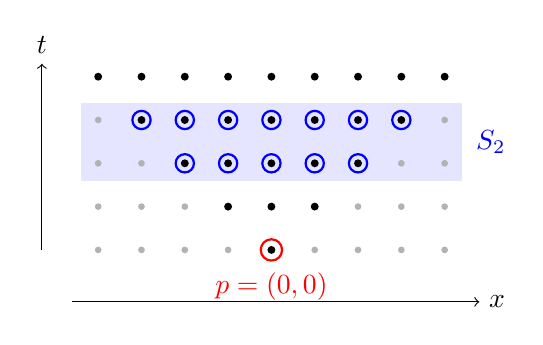
\begin{tikzpicture}[scale=0.55]
  \fill[Blue!10] (-4.4,1.6) rectangle (4.4,3.4);
  \foreach \t in {0,...,4} \foreach \x in {-4,...,4} {
    \pgfmathtruncatemacro{\ax}{abs(\x)}
    \ifnum\ax>\t \fill[gray!60] (\x,\t) circle (2.2pt);
    \else \fill[black] (\x,\t) circle (2.6pt); \fi }
  \foreach \x in {-2,...,2} \draw[Blue,thick] (\x,2) circle (6pt);
  \foreach \x in {-3,...,3} \draw[Blue,thick] (\x,3) circle (6pt);
  \draw[red,thick] (0,0) circle (7pt);
  \node[red,below] at (0,-0.3) {$p=(0,0)$};
  \draw[->] (-5.3,0) -- (-5.3,4.3) node[above] {$t$};
  \draw[->] (-4.6,-1.2) -- (4.8,-1.2) node[right] {$x$};
  \node[Blue,right] at (4.5,2.5) {$S_2$};
\end{tikzpicture}
\caption{The future of $p=(0,0)$ in the lattice $\Z^2$ (black points: $|x|\leq t$) and the
slices $S_2$ (shaded). The circled points form $J(\{p\})\cap S_2$.}
\label{fig:lattice}
\end{figure}

\noindent\motiv{The three relations among sets of lattice points are these. Inclusion
$O\subseteq O'$. Orthogonality: $O_1\perp O_2$ when no point of $O_1$ is comparable with a
point of $O_2$. Dependence: $O\dep O'$ when \revh{for every finite set $Y\subseteq O$} some pair of
slices meets the causal shadow of \revh{$Y$} only inside $O'$, that is, \revh{$J(Y)\cap S_{t_1}\subseteq O'$
for some $t_1$, which may depend on $Y$. Observables will be localized in finite sets, which is why
finite parts of $O$ suffice; for finite $O$ one takes $Y=O$.} For the point $p=(0,0)$:}
\begin{itemize}[leftmargin=2em]
\item \motiv{$\{p\}\perp\{(0,1)\}$ and $\{p\}\perp\{(1,2)\}$, since $|1|>0$ and $|2|>1$;
but $\{p\}$ and $\{(1,1)\}$ are not orthogonal, since $(1,1)$ lies on the future light cone of
$p$.}
\item \motiv{$J(\{p\})\cap S_2$ consists of the points $(2,x)$ with $|x|\leq2$ and $(3,x)$
with $|x|\leq3$ (Figure~\ref{fig:lattice}), so $\{p\}\dep O'$ for every $O'$ containing these
twelve points.}
\item \motiv{$\{p\}\dep\{p\}$ fails: for every $t_1$ the set $J(\{p\})\cap S_{t_1}$ contains at
least four points, \vet{so dependence is not reflexive.}}
\item \motiv{\revh{For the slice $O=\{(0,x):x\in\Z\}$ and $O'=\{(t,x):t\geq1,\ |x|\leq t^2\}$,
$O\dep O'$: a finite $Y\subseteq O$ lies in $|x|\leq R$, and $J(Y)\cap S_{t_1}$ lies in
$|x|\leq R+t_1+1\leq t_1^2$ for large $t_1$. No single pair of slices serves all of $O$, since
$J(O)$ is all of $\Z^2$.}}
\end{itemize}
\end{extra}

\dimockonly{\noindent\motiv{\revm{The regions of spacetime carry three relations that the axioms use: inclusion, orthogonality (spacelike separation) and dependence (one region determines another causally). The definition below keeps only the properties of these relations that the axioms need; Example~\ref{ex:gh-index} is the case of a globally hyperbolic spacetime.}}}


\begin{definition}[Causal index]\label{def:causal-index}
Let $(\cR,\leq)$ be a preordered set, whose elements are called regions. A \emph{causal index}
on $\cR$ consists of two relations, \emph{orthogonality} $O_1\perp O_2$ and \emph{dependence}
$O\dep O'$ (read: $O$ is causally dependent on $O'$), such that for all regions:
\begin{enumerate}[label=(\roman*),leftmargin=2.5em]
\item $O_1\perp O_2$ implies $O_2\perp O_1$;
\item $O_0\leq O_1$ and $O_1\perp O_2$ imply $O_0\perp O_2$;
\item $O_0\leq O$ and $O\dep O'$ imply $O_0\dep O'$;
\item $O\dep O'$ and $O'\leq O_1$ imply $O\dep O_1$.
\end{enumerate}
\end{definition}
From (i) and (ii), orthogonality is also antitone in its second argument: $O_3\leq O_2$ and
$O_1\perp O_2$ imply $O_1\perp O_3$.

\begin{extra}
\begin{example}[The lattice]\label{ex:lattice-index}
The subsets of $\Z^2$ ordered by inclusion, with $\perp$ and $\dep$ as above, form a causal
index. Condition~(i) holds because comparability is symmetric, and (ii) because, for
$O_0\subseteq O_1$, a comparable pair in $O_0\times O_2$ would lie in $O_1\times O_2$. For (iii), \revh{a finite subset of $O_0\subseteq O$ is a finite subset of $O$}. For (iv), enlarging $O'$
preserves the inclusion \revh{$J(Y)\cap S_{t_1}\subseteq O'$}.
\end{example}
\end{extra}

\begin{example}[A globally hyperbolic spacetime]\label{ex:gh-index}
On a globally hyperbolic Lorentzian manifold $(M,g)$ take as regions the open sets with
compact closure. Let $O_1\perp O_2$ when no causal curve joins a point of $O_1$ to a point of
$O_2$; this is \revb{the spacelike separation of~\cite{dimock}}. Let $O\dep O'$ when there is a \revc{smooth spacelike} Cauchy surface
$\Sigma$ such that every endless causal curve through a point of $O$ meets $\Sigma$ in $O'$;
this is the form of causal dependence used in the proof of \revb{Theorem~4 of~\cite[p.~226]{dimock}}.
Conditions (i)--(iv) hold because a causal curve traversed backwards is causal, a curve
through $O_0\subseteq O$ passes through $O$, and a curve meeting $\Sigma$ in $O'$ meets it in
every region containing $O'$.
\end{example}

\begin{remark}[\revm{Dependence through curves}]\label{rem:dimock-dep}
\vet{\revb{The other formulation of~\cite{dimock}}, every endless causal curve through $O$ meets
$O'$~\cite[p.~220]{dimock}, satisfies (i)--(iv) for the same reasons.}
\end{remark}

\begin{extra}
\noindent\motiv{\vet{In the lattice, comparability replaces causal curves and a pair of slices
replaces a Cauchy surface}\revi{, chosen for each finite part of $O$ (Remark~\ref{rem:green-dep-spacetime}
compares the two forms)}\vet{.}}
\end{extra}

\begin{definition}[Isomorphism of causal indices]\label{def:iso}
An \emph{isomorphism} from a causal index on $\cR$ to a causal index on $\cR'$ is a bijection
$\kappa:\cR\to\cR'$ such that $\kappa O\leq\kappa O'\iff O\leq O'$,
$\kappa O_1\perp\kappa O_2\iff O_1\perp O_2$ and $\kappa O\dep\kappa O'\iff O\dep O'$ for all
regions. The isomorphisms of a causal index to itself form a group $\Aut$ under composition,
$(\kappa_1\kappa_2)(O)=\kappa_1(\kappa_2O)$, with the identity as unit.
\end{definition}
Identities, composites and inverses of isomorphisms are isomorphisms, by inspection of the
three equivalences.

\begin{extra}
\begin{example}[Symmetries of the lattice]\label{ex:lattice-aut}
Each point map below sends regions to regions, and the induced map on subsets of $\Z^2$ is an
automorphism of the causal index of Example~\ref{ex:lattice-index}.
\begin{itemize}[leftmargin=2em]
\item A translation $(t,x)\mapsto(t+a,x+b)$ preserves the order of points, hence $J$ and
$\perp$, and maps $S_{t_1}$ to $S_{t_1+a}$.
\item The reflection $(t,x)\mapsto(t,-x)$ preserves the order of points and each slice.
\item The time reversal $(t,x)\mapsto(-t,x)$ reverses the order of points, so it preserves
comparability, $J$ and $\perp$, and maps $S_{t_1}$ to $S_{-t_1-1}$.
\end{itemize}
Regions are ordered by inclusion, which all three maps preserve. \revi{Each map is a bijection of
$\Z^2$ that sends finite sets to finite sets and pairs of slices to pairs of slices, with
$J(\kappa Y)=\kappa J(Y)$, and its inverse is of the same kind, so $\dep$ is preserved in both
directions.}
\end{example}
\end{extra}

\begin{remark}[Time orientation]\label{rem:time-orientation}
\vet{\revo{A time reversal, where the spacetime has one (\extraonly{the lattice of Example~\ref{ex:lattice-aut}, }Minkowski space),} is a symmetry of the causal index. It exchanges the retarded and advanced
propagators of the wave equation~\cite{bgp}, hence $E\mapsto-E$ and $\sigma\mapsto-\sigma$, and by
Remark~\ref{rem:antisymplectic} no $*$-isomorphism sends each Weyl operator $W(u)$ to its time
reverse. Covariance of the free field is therefore required only for maps that preserve the
time orientation.}\extraonly{ \revc{The argument excludes the map of test functions induced by a time
reversal, not every linear map over it: Remark~\ref{rem:massless-reversal} gives a symmetry of the
massless lattice field over the time reversal.}}
\end{remark}

\subsection{Nets and \revd{their axioms}}

\begin{definition}[Net]\label{def:net}
Let $A$ be a C*-algebra and $\cR$ a preordered set. A \emph{net} in $A$ over $\cR$ assigns to
each region $O$ a norm-closed $*$-subalgebra $\cA(O)$ of $A$, the \emph{local algebra} of $O$,
such that $O\leq O'$ implies $\cA(O)\subseteq\cA(O')$ (\emph{isotony}).
\end{definition}
\noindent Each local algebra, being norm closed, is itself a C*-algebra, and it contains the unit of
$A$.

\begin{remark}[The global algebra]\label{rem:global-algebra}
\vet{\revb{In~\cite{dimock} the global algebra is} the closure of the union of the local algebras; here
the net lives in a given algebra $A$, and the generation axiom below states that $A$ is \revo{the C*-algebra generated by the local algebras, which is} that
closure \revo{when the regions are directed (any two lie in a third)}.}
\end{remark}
\noindent\artefact{A net does not carry a causal index; each axiom takes one as an
argument, so that one net can be tested against several causal structures on the same
regions.}

\begin{definition}[The axioms]\label{def:axioms}
Let $\cA$ be a net in $A$ over a causal index on $\cR$.
\begin{enumerate}[label=(N\arabic*),leftmargin=3em]
\item $\cA$ is \emph{generating} if the C*-subalgebra generated by $\bigcup_O\cA(O)$ is $A$.
\item $\cA$ is \emph{causal} if $O_1\perp O_2$ implies $ab=ba$ for all $a\in\cA(O_1)$ and
$b\in\cA(O_2)$.
\item $\cA$ has the \emph{time-slice property} if $O\dep O'$ implies
$\cA(O)\subseteq\cA(O')$.
\end{enumerate}
A representation $\pi:A\to B(H)$ on a complex Hilbert space $H$ is \emph{irreducible} if every
bounded operator $T$ with $T\pi(a)=\pi(a)T$ for all $a\in A$ is a multiple of the identity.
The algebra $A$ is \emph{primitive} if it has an injective irreducible representation on a
nonzero Hilbert space.
\end{definition}
\artefact{The Hilbert spaces allowed in primitivity range over a fixed universe of Hilbert
spaces, determined by $A$. This is no restriction: if $\pi$ is irreducible and $\xi\neq0$, the closure of
$\pi(A)\xi$ is a nonzero closed subspace invariant under $\pi(A)$, and the projection onto it
commutes with $\pi(A)$, so it is the identity and $H=\overline{\pi(A)\xi}$. Hence $H$ has a dense subset indexed by
$A$, and $H$ is unitarily equivalent to a Hilbert space in the universe of $A$.}\par\medskip

\begin{remark}[Irreducibility]\label{rem:irreducible}
\vet{Irreducibility is defined here by a trivial commutant. For representations of C*-algebras
this is equivalent to the absence of closed invariant subspaces other than $0$ and
$H$\revb{ (see, e.g.,~\cite[Ch.~2]{bratteli-robinson-1})}: the commutant of $\pi(A)$ is a von Neumann algebra, so it equals $\C1$ exactly when its
only projections are $0$ and $1$, and its projections are the projections onto closed
invariant subspaces.}
\end{remark}

\begin{remark}[The time-slice axiom]\label{rem:time-slice}
\rev{\revb{Axiom~4 of~\cite[p.~220]{dimock}} reads: if $O$ is causally dependent on $O'$, then
$\cA(O)\subseteq\cA(O')$. \revm{This is (N3) when dependence is taken in the sense of the
spacetime; (N3) for a given causal index is called the time-slice property.} \revb{There} the meaning of causal dependence is left open,
naming as a strong form that every endless causal curve through $O$ meets $O'$
(Remark~\ref{rem:dimock-dep}); \revm{the proof of Theorem~4 of~\cite[p.~226]{dimock} uses}
the form of Example~\ref{ex:gh-index}\revi{; \extraonly{the lattice and }Green data use a pointwise form,
which the form of Example~\ref{ex:gh-index} implies (Remark~\ref{rem:green-dep-spacetime})\revjt{ for the
Green data of Remark~\ref{rem:green-continuum}, and for those of \revm{Chapters~\ref{sec:minkowski}
and~\ref{sec:mass}} when the Cauchy surface is flat (Remark~\ref{rem:mink-slabs})}}. The time-slice axiom of locally
covariant field theory, by which the algebra of a neighbourhood of a Cauchy surface is the
whole algebra, is a different statement\revm{; it is not assumed here}\revo{. For Green data, (N3) gives it for the slabs of the cutoffs, and, for the Green data of Remark~\ref{rem:green-continuum}, for neighbourhoods of every smooth spacelike Cauchy surface (after Theorem~\ref{thm:green-axioms})}.}
\end{remark}

\begin{table}[ht]
\centering\small
\begin{tabular}{@{}ll>{\raggedright\arraybackslash}p{0.36\textwidth}@{}}
\toprule
\revb{Axiom of~\cite[\S1]{dimock}} & content & here \revm{(defined; proved)} \\
\midrule
Axiom 1 & nets of local observables, $\cA=\overline{\bigcup_O\cA(O)}$ &
Definition~\ref{def:net} and (N1)\revm{; Theorems~\ref{thm:weyl-net}} \revo{(for Green data with Proposition~\ref{prop:green-phase}) and}\revm{ \ref{thm:kg-field}} \\
Axiom 2 & primitivity & Definition~\ref{def:axioms}\revf{; Theorem~\ref{thm:primitive}}\revm{, \ref{thm:dimock}} \\
Axiom 3 & first causality (spacelike commutativity) & (N2)\revm{; as for Axiom~1} \\
Axiom 4 & second causality (time slice) & (N3)\revm{; as for Axiom~1, over the causal index at hand} \\
Axiom 5 & covariance & Definition~\ref{def:covariance}\revm{; Theorems~\ref{thm:ccr-cov}, \extraonly{\ref{thm:lattice-net}, }\ref{thm:mink-covariance}, \ref{thm:kg-field}(c)} \\
\bottomrule
\end{tabular}
\caption{\revb{The axioms of~\cite{dimock}} and \revg{where they are defined or proved}.}
\label{tab:dimock}
\end{table}

\begin{definition}[Covariance]\label{def:covariance}
Let $\cA$ be a net in $A$ over a causal index on $\cR$, and $\cA'$ a net in $A'$ over a causal
index on $\cR'$. A pair $(\kappa,\alpha)$ of an isomorphism $\kappa$ of the causal indices and
a $*$-isomorphism $\alpha:A\to A'$ is a \emph{covariance pair} from $\cA$ to $\cA'$ if
\begin{equation}\label{eq:covariance}
\alpha\bigl(\cA(O)\bigr)=\cA'(\kappa O)\qquad\text{for every region }O.
\end{equation}
Two nets over the same causal index are \emph{isomorphic} if some $(\mathrm{id},\alpha)$ is a
covariance pair between them. A net $\cA$ is \emph{covariant under} a group $\Gamma$, given
group homomorphisms $\gamma\mapsto\kappa_\gamma$ into $\Aut$ and $\gamma\mapsto\alpha_\gamma$
into the $*$-automorphisms of $A$, if each $(\kappa_\gamma,\alpha_\gamma)$ is a covariance
pair from $\cA$ to itself.
\end{definition}

\begin{lemma}[Covariance pairs compose]\label{lem:pairs}
The pair $(\mathrm{id},\mathrm{id})$ is a covariance pair from a net to itself. If
$(\kappa_1,\alpha_1)$ is a covariance pair from $\cA$ to $\cA'$ and $(\kappa_2,\alpha_2)$ one
from $\cA'$ to $\cA''$, then $(\kappa_2\circ\kappa_1,\alpha_2\circ\alpha_1)$ is one from $\cA$
to $\cA''$, and $(\kappa_1^{-1},\alpha_1^{-1})$ is one from $\cA'$ to $\cA$.
\end{lemma}
\begin{proof}
The first claim is~\eqref{eq:covariance} for identities. For the second,
$\alpha_2\alpha_1(\cA(O))=\alpha_2(\cA'(\kappa_1O))=\cA''(\kappa_2\kappa_1O)$. For the third,
put $O=\kappa_1^{-1}O'$ in $\alpha_1(\cA(O))=\cA'(\kappa_1O)$ and apply $\alpha_1^{-1}$:
$\cA(\kappa_1^{-1}O')=\alpha_1^{-1}(\cA'(O'))$.
\end{proof}

\begin{remark}[Covariance as an assignment]\label{rem:axiom5}
\vet{\revb{Axiom~5 of~\cite{dimock}} asks for more than a single pair: an assignment
$\kappa\mapsto\alpha_\kappa$ on the isometries between spacetimes of one isometry class, with
$\alpha_{\mathrm{id}}=\mathrm{id}$ and $\alpha_{\kappa_1\kappa_2}=\alpha_{\kappa_1}
\alpha_{\kappa_2}$, each $(\kappa,\alpha_\kappa)$ a covariance pair. Such an assignment is a
construction on a family of nets. By Lemma~\ref{lem:pairs},
$(\kappa_1\kappa_2,\alpha_{\kappa_1}\alpha_{\kappa_2})$ is a covariance pair whenever the
factors are, so the composition law compares two covariance pairs over the same
isometry~$\kappa_1\kappa_2$.}
\end{remark}

\subsection{Nets generated by families of elements}

\noindent\motiv{The local algebras of the free field are generated by explicit unitaries, the
Weyl operators of test functions localized in the region. Whether two such algebras commute is
therefore a question about their generators. The answer needs one more hypothesis than the
commutation of the generators themselves\extraonly{ \vet{(Examples~\ref{ex:two-qubits}
and~\ref{ex:nilpotent})}}.}

\begin{extra}
\begin{example}[Two qubits]\label{ex:two-qubits}
In $A=M_2(\C)\otimes M_2(\C)$ let $s=\{\sigma_x\otimes1,\sigma_z\otimes1\}$ and
$s'=\{1\otimes\sigma_x,1\otimes\sigma_z\}$. Since
$\sigma_x\sigma_z=-\ii\sigma_y$, the $*$-algebra generated by $\sigma_x,\sigma_z$ contains
$1,\sigma_x,\sigma_y,\sigma_z$, which span $M_2(\C)$. Hence $\calg(s)=M_2(\C)\otimes1$ and
$\calg(s')=1\otimes M_2(\C)$, and every element of the first commutes with every element of the
second.
\end{example}
\end{extra}

\begin{extra}
\begin{example}[An element commuting with itself]\label{ex:nilpotent}
In $A=M_2(\C)$ let $e=\begin{psmallmatrix}0&1\\0&0\end{psmallmatrix}$ and $s=s'=\{e\}$. Every
element of $s$ commutes with every element of $s'$. But $ee^*=\begin{psmallmatrix}1&0\\0&0
\end{psmallmatrix}$ and $e^*e=\begin{psmallmatrix}0&0\\0&1\end{psmallmatrix}$, so $e$ does not
commute with $e^*$, and $\calg(s)$, which contains $e$ and $e^*$, is all of $M_2(\C)$ and is not
commutative. The generated algebras do not commute.
\end{example}
\end{extra}

\noindent\motiv{\extraonly{\vet{Commutation with adjoints is the hypothesis that
Example~\ref{ex:nilpotent} lacks.} }For a subset \revi{$s$} of $A$ let
\[
Z(\revi{s})=\{x\in A:\ xb=bx\ \text{and}\ xb^*=b^*x\ \text{for all }b\in \revi{s}\},
\]
the elements commuting with every element of \revi{$s$} and with its adjoint.}

\begin{lemma}[Commutation of generated algebras]\label{lem:commute}
Let \revk{$A$ be a C*-algebra and} $s,s'\subseteq A$, and suppose that every $a\in s$ commutes with every $b\in s'$ and with
every $b^*$, $b\in s'$. Then every element of $\calg(s)$ commutes with every element of
$\calg(s')$.
\end{lemma}
\begin{proof}
The set \revi{$Z(s)$} is a C*-subalgebra of $A$ for every \revi{$s$}. It is a unital subalgebra. It is closed
under the adjoint: taking adjoints in $xb=bx$ and $xb^*=b^*x$ gives $b^*x^*=x^*b^*$ and
$bx^*=x^*b$. It is norm closed, since each equation $xb=bx$ survives norm limits.

The hypothesis says $s\subseteq Z(s')$, so $\calg(s)\subseteq Z(s')$. Fix $x\in\calg(s)$. Both
$x$ and $x^*$ lie in $\calg(s)\subseteq Z(s')$, so every $b\in s'$ commutes with $x$ and with
$x^*$; that is, $s'\subseteq Z(\{x\})$. Hence $\calg(s')\subseteq Z(\{x\})$, and every element of
$\calg(s')$ commutes with $x$.
\end{proof}
\extraonly{In Example~\ref{ex:two-qubits} every generator is self-adjoint, so the hypothesis reduces to
commutation of the generators. In Example~\ref{ex:nilpotent} it fails, because $e$ does not
commute with $e^*$.}

\begin{definition}[Generated net]\label{def:generated}
A \emph{family of generators} in $A$ over $\cR$ assigns to each region $O$ a subset $G(O)$ of
$A$, with $G(O)\subseteq G(O')$ whenever $O\leq O'$. The net \emph{generated} by $G$ is
$\cA_G(O)=\calg(G(O))$.
\end{definition}
It is a net: each $\calg(G(O))$ is a norm-closed $*$-subalgebra, and $s_0\subseteq s_1$ implies
$\calg(s_0)\subseteq\calg(s_1)$.

\begin{proposition}[Axioms from generators]\label{prop:generated}
Let $G$ be a family of generators in \revk{a C*-algebra} $A$ over a causal index on \revk{a
preordered set} $\cR$ \revk{of regions}.
\begin{enumerate}[label=(\alph*),leftmargin=2.5em]
\item If, whenever $O_1\perp O_2$, every $a\in G(O_1)$ commutes with every $b\in G(O_2)$ and
with every $b^*$, $b\in G(O_2)$, then $\cA_G$ is causal.
\item If\revf{, whenever} $O\dep O'$\revf{,} $G(O)\subseteq\cA_G(O')$, then $\cA_G$ has the time-slice
property.
\item If $\calg\bigl(\bigcup_OG(O)\bigr)=A$, then $\cA_G$ is generating.
\item Let $G'$ be a family of generators in $A'$ over a causal index on $\cR'$, $\kappa$ an
isomorphism of the causal indices and $\alpha:A\to A'$ a $*$-isomorphism with
$\alpha(G(O))=G'(\kappa O)$ for every $O$. Then $(\kappa,\alpha)$ is a covariance pair from
$\cA_G$ to $\cA_{G'}$.
\end{enumerate}
\end{proposition}
\begin{proof}
\begin{enumerate}[leftmargin=2.5em]
\item[(a)] Lemma~\ref{lem:commute} with $s=G(O_1)$ and $s'=G(O_2)$.
\item[(b)] $\cA_G(O')$ is a C*-subalgebra containing $G(O)$, hence it contains $\calg(G(O))$.
\item[(c)] The C*-subalgebra generated by $\bigcup_O\cA_G(O)$ contains $\bigcup_OG(O)$, hence
contains $\calg(\bigcup_OG(O))=A$.
\item[(d)] A $*$-homomorphism maps the $*$-algebra generated by a set onto the $*$-algebra generated
by its image, so $\alpha(\alg(G(O)))=\alg(G'(\kappa O))$. It remains to pass to closures. A
$*$-homomorphism $\varphi$ between C*-algebras does not increase norms: the spectrum of
$\varphi(b)$ is contained in that of $b$, the norm of a self-adjoint element is its spectral
radius, and so $\|\varphi(a)\|^2=\|\varphi(a^*a)\|\leq\|a^*a\|=\|a\|^2$. Applied to $\alpha$ and
$\alpha^{-1}$, this makes $\alpha$ a homeomorphism, which maps the closure of a set onto the
closure of its image. Hence $\alpha(\calg(G(O)))=\calg(G'(\kappa O))$.
\end{enumerate}
\end{proof}

\begin{remark}[\revm{Moving generators}]\label{rem:weak-time-slice}
In (b) the generators of $O$ are required to lie in the closed algebra of $O'$, not in $G(O')$.
\rev{For the free field the Weyl operators are labelled by the classes $[f]$ of test
functions modulo the kernel of $E$ (Remark~\ref{rem:dictionary}), and the stronger inclusion
holds: if $O\dep O'$, every $f$ localized in $O$ has an $f'$ localized in $O'$ with $Ef'=Ef$\extraonly{ (on
the lattice this is Corollary~\ref{cor:lattice-dep})}, so $[f]=[f']$ and the generator
$W([f])$ of $O$ is a generator of $O'$. This is the step of the proof of \revb{Theorem~4
of~\cite[p.~226]{dimock}} that gives time slice. \revd{The classes and the net are constructed in Chapter~\ref{sec:phasespace}
(\extraonly{Example~\ref{ex:lattice-phase} and }Definition~\ref{def:weyl-net}).}}
\end{remark}
